\documentclass[11pt,letterpaper,dvipsnames]{article}
\usepackage{fullpage}
\usepackage{multicol}
\usepackage{amsmath}
\usepackage{amsfonts}
\usepackage{amssymb}
\usepackage{amsthm}
\usepackage{graphicx, nicefrac}
\usepackage{tikz, nicefrac}

\newenvironment{solution}{\color{SeaGreen}\textit{Solution.}}{\color{black}}

\newcommand{\ds}{\displaystyle}
\newcommand{\bv}{\mathbf}
\newcommand{\lv}{\langle}
\newcommand{\rv}{\rangle}

\begin{document}

\flushleft

\begin{center}
    \begin{large}
        \textbf{Homework 5} \\
        MAD4204 \\ 
        Carson Mulvey
    \end{large}
\end{center}

\pagestyle{empty}


\flushleft
\begin{enumerate}

\item Let $P = [2] \times [3]$, where we view $[n]$ as a chain.
\begin{enumerate}
	\item Draw the poset $J(P)$ and find its join irreducibles.
	\item Show that $P$ and $J(P)$ are ranked and find their rank generating functions.
	\item Find all the linear extensions of $P$ (Bonus: do this for $J(P)$ too!).
	\item Compute $\mu(\hat{0},\hat{1})$ for $J(P)$.
\end{enumerate}
\begin{solution}
\begin{enumerate}
    \item Denoting $(a,b)$ as $ab$ for shorthand, we see that $J(P)=$ 
    
    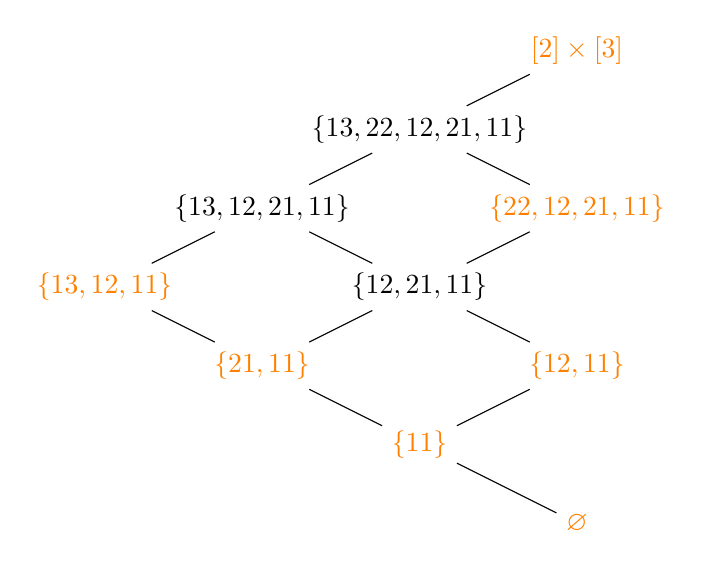
\begin{tikzpicture}
        \node[orange] (min) at (6,0) { $\varnothing$};
        \node[orange] (a) at (4,1) {$\{11\}$};
        \node[orange] (b) at (2,2) {$\{21,11\}$};
        \node[orange] (c) at (6,2) {$\{12,11\}$};
        \node[orange] (d) at (0,3) {$\{13,12,11\}$};
        \node (e) at (4,3) {$\{12,21,11\}$};
        \node (f) at (2,4) {$\{13,12,21,11\}$};
        \node[orange] (g) at (6,4) {$\{22,12,21,11\}$};
        \node (h) at (4,5) {$\{13,22,12,21,11\}$};
        \node[orange] (max) at (6,6) {$[2]\times[3]$};
        \draw (min) -- (a) -- (c) -- (e) -- (g) -- (h) -- (max)
        (a) -- (b) -- (e) -- (f) -- (h)
        (b) -- (d) -- (f);
    \end{tikzpicture}
    
    with {\color{orange} orange} sets being its join irreducibles.
    
    \item Since $P$ essentially creates a 1x2 block-walking grid, $P$ has $3$ maximal chains, all of length $3$. In $J(P)$, a maximal chain is a path from $\varnothing$ to $[2]\times[3]$. Since an element is added at each step in the path, all maximal chains have length $6$. Thus, both $P$ and $J(P)$ are ranked. In particular, 
    \begin{align*}
        F_P(q) &= 1+2q+2q^2+q^3, \\
        F_{J(P)}(q) &= 1+q+2q^2+2q^3+2q^4+q^5+q^6.
    \end{align*}
    
    \item For any linear extension $L$, clearly $L(11)=1$ and $L(23)=6$. We can casework by $L(12)\in\{2,3\}$ to get all linear extensions as follows:
    \begin{center}\begin{tabular}{ c|cccccc } 
$i$ & $L_i(11)$ & $L_i(12)$ & $L_i(21)$ & $L_i(13)$ & $L_i(22)$ & $L_i(23)$\\
\hline
1 & 1 & 2 & 3 & 5 & 4 & 6 \\ 
2 & 1 & 2 & 3 & 4 & 5 & 6 \\ 
3 & 1 & 2 & 4 & 3 & 5 & 6 \\ 
4 & 1 & 3 & 2 & 4 & 5 & 6 \\ 
5 & 1 & 3 & 2 & 5 & 4 & 6 \\
\end{tabular}\end{center}
    \item We have $\mu(\hat{0},\hat{0})=1$, so $\mu(\hat{0},\{11\})=-\mu(\hat{0},\hat{0})=-1$. Then
    \begin{align*}
        \mu(\hat{0},\{21,11\})&=\mu(\hat{0},\{12,11\}) \\
        &=\mu(\hat{0},\hat{0})+\mu(\hat{0},\{11\}) \\
        &=0.
    \end{align*}
    Continuing this process recursively, we see that $\mu(\hat{0},p)=0$ for any $p\in{P}$ with rank greater than $1$. Thus $\mu(\hat{0},\hat{1})=0$.

\end{enumerate}
\end{solution}

\item Let $L$ be a finite lattice. Show  $x \wedge (y \vee z) = (x \wedge y) \vee (x \wedge z)$ for all $x,y,z \in L$ if and only if $x \vee (y \wedge z) = (x \vee y) \wedge (x \vee z)$ for all $x,y,z \in L$.


(A lattice satisfying either of these properties is called a \emph{distributive lattice}.)

\begin{solution}
    $(\implies)$ Assume that $\wedge$ distributes over $\vee$. Then
    \begin{align*}
        (x\vee y)\wedge (x\vee z) &= ((x\vee y)\wedge x)\vee ((x\vee y)\wedge z) \\
        &= x \vee  ((x\vee y)\wedge z) \\
        &= x \vee (z \wedge (x\vee y)) \\
        &= x \vee ((z \wedge x) \vee (z \wedge y)) \\
        &= (x \vee (z \wedge x)) \vee (z \wedge y) \\
        &= x \vee (z \wedge y)
    \end{align*}
as desired.

    $(\impliedby)$ Now assume that $\vee$ distributes over $\wedge$. We let $\tilde{L}$, the \textit{dual} of $L$, be the lattice where $p\leq_L{q} \iff q\leq_{\tilde{L}}{p}$. We see that $\tilde{L}$ is indeed a lattice, since $\vee_L=\wedge_{\tilde{L}}$ and $\wedge_L=\vee_{\tilde{L}}$. Using this duality, $(\impliedby)$ for $L$ is equivalent to $(\implies)$ for $\tilde{L}$, so we are done. \qed
\end{solution}

\item Let $L$ be a finite distributive lattice. 
For $t \in L$, let $K_t = \{p \in \mbox{Irr}(L): p \leq t\}$.
Show
\[
t = \bigvee_{p \in K_t} p.
\]

\begin{solution}
    Since $p\leq t$ for all $p\in K_t$, by Proposition 16.29, $\bigvee_{p \in K_t} p \leq t$. However, since all of $p$ are join irreducible, $t \leq \bigvee_{p \in K_t} p$. Thus
    \[
t = \bigvee_{p \in K_t} p.
\]
\qed
\end{solution}

\item 
In class we introduced Young's lattice $Y$, which is equivalent to the subposet of finite ideals in $J(\mathbb{N} \times \mathbb{N})$ or partitions ordered under containment of Young diagrams.
\begin{enumerate}
\item Show $Y$ is a distributive lattice and describe $\mbox{Irr}(Y)$ (Hint: what are $\wedge$ and $\vee$?).
\item Let $\lambda = \mu^1 \vee \dots \vee \mu^k$ where $\{\mu^1,\dots,\mu^k\} \subset \mbox{Irr}(Y)$ is an antichain.
Give a combinatorial interpretation of $k$ in terms of properties of $\lambda$.
\end{enumerate}

\begin{solution}
\begin{enumerate}
    \item Because $\wedge$ and $\vee$ are the intersection and union of Young diagrams, respectively, and these operations are distributive, $Y$ must be a distributive lattice.
    
    Since join irreducibles must cover at most one element, $\mbox{Irr}(Y)$ will contain the empty set, as well as for any integer $n>0$, partitions of singleton $n$, as well as the partition $\underbrace {1+\cdots +1} _{n{\text{ times}}}$.
    
    \item Since partitions of singleton $n$ as described above contain one another, at most one can be chosen to form an antichain. Similarly, partitions of form $\underbrace {1+\cdots +1} _{n{\text{ times}}}$ must contain one another, so at most one can be chosen for an antichain. Then $k$ is at most $2$, and $\lambda$ takes form $n+\underbrace {1+\cdots +1} _{m{\text{ times}}}$ for $n,m\in{\mathbb{N}}$.
\end{enumerate}
\end{solution}

\end{enumerate}
\end{document}